\subsection{Tworzenie okien}
\label{netTworzenieOkien}

Przypomnijmy sobie najprostszy program ze strony \pageref{tworzenieOkienAPI}, który tworzył zwykłe, 
proste okno na pulpicie. Jego odpowiednik w świecie .NET wygląda tak:

\begin{scriptsize}
\begin{verbatim}
/* Wiktor Zychla, 2003 */
using System;
using System.Windows.Forms;

namespace Example
{
  public class CMainForm : Form
  {   
    public CMainForm()
    {
      this.Text = "Okna w świecie .NET"; 
    }

    public static void Main()
    {
      Application.Run( new CMainForm() );
    }
  }
}
\end{verbatim}
\end{scriptsize}

Różnica w przejrzystości programu jest kolosalna! Interfejs biblioteki {\bf System.Windows.Forms} jest
w pełni obiektowy. Utworzenie okna polega po prostu na utworzeniu klasy dziedziczącej z klasy
{\bf Form}. Klasa ta zamyka w sobie całą funkcjonalność jakiej potrzeba aby obsłużyć proste okno: obiekt
który utworzyliśmy w przykładowym programie powyżej ma kilkadziesiąt propercji i metod oraz obsługuje
kilkadziesiąt zdarzeń.

Powyższy kod może w pierwszej chwili wydawać się dość zaskakujący, bowiem nie ma tu nigdzie
pętli obsługi komunikatów. Okazuje się, że pętla obsługi komunikatów jest ukryta w funkcji
{\bf Run} klasy {\bf Application}. Dodatkowym, opcjonalnym parametrem metody {\bf Run} jest
obiekt, będący {\em głównym oknem aplikacji}. Aplikacja automatycznie zakończy się, kiedy główne
okno aplikacji zostanie zniszczone.

Oczywiście taka konstrukcja utrudnia nieco sterowanie aplikacją wtedy, gdy powinna ona
zajmować się czymś oprócz przetwarzania komunikatów. 
Na stronie \pageref{apiPetlaObslugiKomunikatow} widzieliśmy jak radzić sobie z takim problemem w Win32Api
(zamiast {\bf GetMessage} użyliśmy {\bf PeekMessage}),
zaś na stronie \pageref{netPetlaObslugiKomunikatow} pokazano jak wygląda analogiczna konstrukcja
w świecie .NET.

Widać również, że programista w przeciwieństwie do Win32API nie musi samodzielnie 
rejestrować klasy okna w systemie. Właściwości klasy okna opisuje definicja klasy, zaś sama operacja
rejestrowania klasy okna w systemie odbywa się bez udziału programisty\footnote{W świecie
.NET definicja okna jest klasą. Aby takie okno mogło pojawić się w systemie, w systemie rejestrowana jest
oczywiście klasa okna. Nie należy jednak mylić tych dwóch pojęć i dlatego wprowadzimy dwa różne określenia:
{\em klasą okna} będziemy nazywać obiekt systemowy, opisujący właściwości okna i rejestrowany w systemie
za pomocą funkcji {\bf RegisterClass}, zaś {\em klasą opisującą okno}, będziemy nazywać definicję
klasy dziedziczącej z klasy {\bf Form}, opisującej właściwości okna w C\#.}.

\subsection{Okna potomne}

W obiektowym świecie {\bf System.Windows.Forms}, każdy obiekt dziedziczący z klasy {\bf Control} (klasa
{\bf Form} dziedziczy z klasy {\bf Control} i jest od niej odległa o 4 pokolenia) ma propercję
{\bf Controls}, która zwraca kolekcję okien potomnych względem tego obiektu. Oznacza to, że
okna potomne mogą być łatwo tworzone w czasie działania programu. Te okna potomne, które powinny
być widoczne od razu po utworzeniu okna można utworzyć po prostu w konstruktorze okna macierzystego.

Najwygodniej jest uczynić okna potomne polami składowymi klasy opisującej okno macierzyste. Wtedy wszystkie
inne składowe klasy okna macierzystego mają dostęp do okien potomnych. Okna potomne są również obiektami,
podlegają więc dokładnie takim samym prawom jak wszystkie obiekty - muszą być jawnie
skonstruowane, są odśmiecane itd.

\begin{figure}
\begin{center}
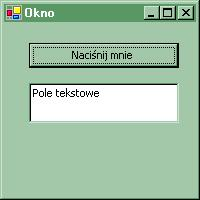
\includegraphics[width=0.30\textwidth]{./pic/n01}
\caption{Proste okno w świecie .NET}
\end{center}
\end{figure}

\begin{scriptsize}
\begin{verbatim}
/* Wiktor Zychla, 2003 */
using System;
using System.Drawing;
using System.Windows.Forms;

namespace Example
{
  public class CMainForm : Form
  {   
    Button  btOK;
    TextBox pTxt;   

    public CMainForm()
    {
      btOK           = new Button();     
      btOK.Location  = new Point( 25, 20 );
      btOK.Size      = new Size( 150, 25 );
      btOK.Text      = "Naciśnij mnie";

      pTxt           = new TextBox();
      pTxt.Location  = new Point( 25, 60 );
      pTxt.Size      = new Size( 150, 40 );
      pTxt.Multiline = true;
      pTxt.Text      = "Pole tekstowe";

      this.Controls.AddRange( new Control[] { btOK, pTxt } );

      this.Text = "Okno"; 
      this.Size = new Size( 200, 200 );
    }

    public static void Main()
    {
       Application.Run( new CMainForm() );
    }
  }
}
\end{verbatim}
\end{scriptsize}

Tworząc okna można zejść aż na poziom równy funkcji {\bf CreateWindow}, na którym można utworzyć
okno podając nazwę klasy okna, jego styl i rozmiary.

\begin{scriptsize}
\begin{verbatim}
/* Wiktor Zychla, 2003 */
using System;
using System.Drawing;
using System.Windows.Forms;

namespace Example
{
  public class CMainForm : Form
  {   
    const int WS_VISIBLE = 0x10000000;
    const int WS_CHILD   = 0x40000000;

    public CMainForm()
    {
      CreateParams cp = new CreateParams();
      cp.ClassName  = "EDIT";      
      cp.Style      = WS_CHILD | WS_VISIBLE;
      cp.Parent     = this.Handle;
      cp.Width      = 150;
      cp.Height     = 25;
      cp.X          = 20;
      cp.Y          = 20; 

      NativeWindow t = new NativeWindow();
      t.CreateHandle( cp );

      this.Text = "Okno"; 
      this.Size = new Size( 200, 200 );      
    }

    public static void Main()
    {
       Application.Run( new CMainForm() );
    }
  }
}
\end{verbatim}
\end{scriptsize}

\subsection{Zdarzenia}

W rozdziale \ref{delegaciZdarzenia} na stronie \pageref{delegaciZdarzenia} widzieliśmy w jaki sposób
C\# rozwiązuje problem zdarzeń. Dzięki temu, że zdarzenie jest tak naprawdę listą odpowiednich delegatów,
zajście zdarzenia może śledzić dowolna ilość słuchaczy.

Taki model doskonale sprawda się w aplikacjach okienkowych, gdzie tak naprawdę istotne są
właśnie reakcje na zdarzenia zgłaszane do okien aplikacji. Aby okna reagowały na działania użytkownika, wystarczy 
więc pod odpowiednie zdarzenia "przypiąć"ich słuchaczy. Zdarzenia udostępniane przez komponenty wizualne
dość dobrze odpowiadają komunikatom, jakie komponenty te mogłyby obsługiwać. 

\begin{scriptsize}
\begin{verbatim}
/* Wiktor Zychla, 2003 */
using System;
using System.Drawing;
using System.Windows.Forms;

namespace Example
{
  public class CMainForm : Form
  {   
    Button  btOK;
    TextBox pTxt;   

    public CMainForm()
    {
      btOK           = new Button();     
      btOK.Location  = new Point( 25, 20 );
      btOK.Size      = new Size( 150, 25 );
      btOK.Text      = "Naciśnij mnie";

      pTxt           = new TextBox();
      pTxt.Location  = new Point( 25, 60 );
      pTxt.Size      = new Size( 150, 40 );
      pTxt.Multiline = true;
      pTxt.Text      = "Pole tekstowe";

      // dodaj zdarzenia
      btOK.Click    += new EventHandler( btOk_Click );
      pTxt.KeyPress += new KeyPressEventHandler( pTxt_KeyPress );

      this.Controls.AddRange( new Control[] { btOK, pTxt } );

      this.Text = "Okno"; 
      this.Size = new Size( 200, 200 );
    }

    void btOk_Click( object sender, EventArgs e )
    {
      MessageBox.Show( "Kliknięto przycisk" ); 
    }

    void pTxt_KeyPress( object sender, KeyPressEventArgs e )
    {
      this.Text = e.KeyChar.ToString();
    }

    public static void Main()
    {
       Application.Run( new CMainForm() );
    }
  }
}
\end{verbatim}
\end{scriptsize}

Wśród ważniejszych zdarzeń warto wymienić:
\begin{itemize}
\item Click
\item DoubleClick
\item Enter
\item KeyDown
\item KeyPress
\item KeyUp
\item Leave
\item MouseDown
\item MouseHover
\item MouseUp
\item Move
\item Paint
\item Resize
\item Validating
\item Validated
\end{itemize}

\subsubsection{Parametry zdarzeń}

Przy tak dużej ilości zdarzeń pojawiają się różne problemy. Na przykład - 
różne zdarzenia mogą mieć różne ilości parametrów. Informacja o naciśnięciu klawisza
powinna nieść ze sobą informację o tym klawiszu, zaś informacja o naciśnięciu przycisku myszy powinna mówić
który przycisk został naciśnięty i jaka jest pozycja wskaźnika w oknie. Ponadto, gdyby jedna i ta sama
funkcja została przypisana do obsługi różnych zdarzeń różnych komponentów, to wewnątrz funkcji obsługującej
to zdarzenie zdecydowanie powinno dać się określić ten komponent, który spowodował powstanie zdarzenia.

Na szczęście te problemy rozwiązano dość elegancko. Przyjęto konwencję, wedle której obiekt będący
źródłem zdarzenia przekazuje się zawsze jako pierwszy parametr do delegata reagującego na zajście zdarzenia,
zaś parametry zdarzenia przekazuje się w obiektach klas dziedziczących z klasy {\bf EventArgs} jako drugi
parametr tych delegatów. Na przykład zdarzenie naciśnięcia
klawisza przekazuje swoje parametry w obiekcie typu {\bf KeyPressEventArgs}, zaś zdarzenia myszy w
obiektach typu {\bf MouseEventArgs}. 

Oznacza to, że wszyscy delegaci będący słuchaczami zdarzeń związanych z obsługą komponentów wizualnych mają
bardzo podobną postać. Nazwy tych delegatów i nazwy ich parametrów odpowiadają nazwom odpowiednich zdarzeń.

\begin{scriptsize}
\begin{verbatim}
delegate void EventHandler( object sender, EventArgs e );
delegate void KeyPressEventHandler( object sender, KeyPressEventArgs e );
...
\end{verbatim}
\end{scriptsize}

\subsubsection{Pokrywanie funkcji obsługi zdarzeń}

Oprócz możliwości przypinania słuchaczy do odpowiednich zdarzeń, istnieje możliwość
przeciążenia funkcji wirtualnych dziedziczonych z klasy {\bf Control}, będących reakcjami na zdarzenia.
W tym przypadku funkcja ma już tylko jeden parametr, określający parametry zdarzenia.

\begin{scriptsize}
\begin{verbatim}
/* Wiktor Zychla, 2003 */
using System;
using System.Drawing;
using System.Windows.Forms;

namespace Example
{
  public class CMyButton : Button
  {
    protected override void OnClick( EventArgs e )
    {
      base.OnClick( e ); 
      MessageBox.Show( "Kliknięto mnie!" );
    } 
  }

  public class CMainForm : Form
  {   
    public CMainForm()
    {
      CMyButton btOK;       

      btOK           = new CMyButton();     
      btOK.Location  = new Point( 25, 20 );
      btOK.Size      = new Size( 150, 25 );
      btOK.Text      = "Naciśnij mnie";

      this.Controls.Add( btOK );

      this.Text = "Okno"; 
      this.Size = new Size( 200, 200 );
    }

    public static void Main()
    {
       Application.Run( new CMainForm() );
    }
  }
}
\end{verbatim}
\end{scriptsize}

Nic nie stoi na przeszkodzie, aby równolegle dodać funkcje reagujące na to samo zdarzenie do odpowiedniej
listy delegatów (przy okazji zwróćmy uwagę na to w jakiej kolejności wywołają się 
oba zdarzenia. Od czego to zależy?):

\begin{scriptsize}
\begin{verbatim}
/* Wiktor Zychla, 2003 */
using System;
using System.Drawing;
using System.Windows.Forms;

namespace Example
{
  public class CMyButton : Button
  {
    protected override void OnClick( EventArgs e )
    {
      base.OnClick( e ); 
      MessageBox.Show( "Kliknięto mnie!" );
    } 
  }

  public class CMainForm : Form
  {   
    public CMainForm()
    {
      CMyButton btOK;       

      btOK           = new CMyButton();     
      btOK.Location  = new Point( 25, 20 );
      btOK.Size      = new Size( 150, 25 );
      btOK.Text      = "Naciśnij mnie";

      btOK.Click += new EventHandler( btOK_Click );

      this.Controls.Add( btOK );

      this.Text = "Okno"; 
      this.Size = new Size( 200, 200 );
    }

    public void btOK_Click( object sender, EventArgs e )
    {
      MessageBox.Show( "I znów mnie kliknięto!" );
    }

    public static void Main()
    {
       Application.Run( new CMainForm() );
    }
  }
}
\end{verbatim}
\end{scriptsize}

Powstaje więc pytanie: gdzie w takim razie określać reakcje na zdarzenia, czy przeciążając odpowiednią 
funkcję czy dokładając delegata do listy słuchaczy zdarzenia?

Odpowiedź wbrew pozorom jest dość prosta: przeciążanie funkcji obsługi zdarzenia powinno stosować się tylko
tam, gdzie reakcja na zdarzenie powinna być taka sama dla {\em wszystkich} instancji tworzonego komponentu i 
w dodatku powinna być jego trwałą właściwością. Takiej funkcji nie można już bowiem odwołać. 

Jeśli zaś reakcja na zdarzenie ma być wewnętrzną sprawą jakiejś konkretnej {\em instancji} komponentu, tam
reakcja ta powinna być delegatem na liście słuchaczy zdarzenia.

\subsection{Okna dialogowe}

Skoro okna w świecie .NET są instancjami odpowiednich klas, to tworzenie nowych okien jest tak proste
jak wykreowanie nowych obiektów. Po wykreowaniu okno może być pokazane jako modalne za pomocą metody
{\bf ShowDialog} lub jako niemodalne za pomocą {\bf Show}.

\begin{scriptsize}
\begin{verbatim}
/* Wiktor Zychla, 2003 */
using System;
using System.Drawing;
using System.Windows.Forms;

namespace Example
{
  public class CSecondaryForm : Form
  {
    public CSecondaryForm()
    {
      this.Text = "Okno dialogowe";
    }
  }

  public class CMainForm : Form
  {   
    public CMainForm()
    {
      Button btOK;       

      btOK           = new Button();     
      btOK.Location  = new Point( 25, 20 );
      btOK.Size      = new Size( 150, 25 );
      btOK.Text      = "Pokaż okno dialogowe";

      btOK.Click += new EventHandler( btOK_Click );

      this.Controls.Add( btOK );

      this.Text = "Okno"; 
      this.Size = new Size( 200, 200 );
    }

    public void btOK_Click( object sender, EventArgs e )
    {
      CSecondaryForm f = new CSecondaryForm();
      f.ShowDialog(); 
    }

    public static void Main()
    {
      Application.Run( new CMainForm() );
    }
  }
}
\end{verbatim}
\end{scriptsize}

Klasa opisująca okno może mieć dowolną ilość konstruktorów, których można użyć do przekazania
parametrów nowo tworzonym oknom.

